\documentclass[dvipdfmx,8pt]{beamer}


\usepackage{here, amsmath, latexsym, amssymb, bm, ascmac, mathtools, multicol, tcolorbox, subfig, color, tikz, graphics, braket}
\usepackage{pxjahyper}%しおりの文字化けを防ぐ
\renewcommand{\baselinestretch}{1.2}
\renewcommand{\figurename}{図}
\renewcommand{\tablename}{表}
\renewcommand{\kanjifamilydefault}{\gtdefault}
\usefonttheme{professionalfonts}
\setbeamertemplate{navigation symbols}{}

\usetheme{Boadilla}

\title{ディープラーニングと物理学}
\subtitle{4.3 \ LSTM}
\author[須賀]{須賀勇貴}
\institute[茨大]{茨城大学大学院 \ 理工学研究科 \ 量子線科学専攻 \ 2年}
\date{\today}

\begin{document}

\frame{\maketitle}
  \section{LSTMの構造}
  \begin{frame}{LSTMの構造}
    \begin{block}{LSTM(Long short-term memory)}
      RNNの中間層のユニットをメモリー・ユニットに置き換えもの\\
      メモリー・ユニットには情報の保持や忘却を可能にする仕組みが組み込まれている      
    \end{block}
    \begin{figure}
      \begin{center}
        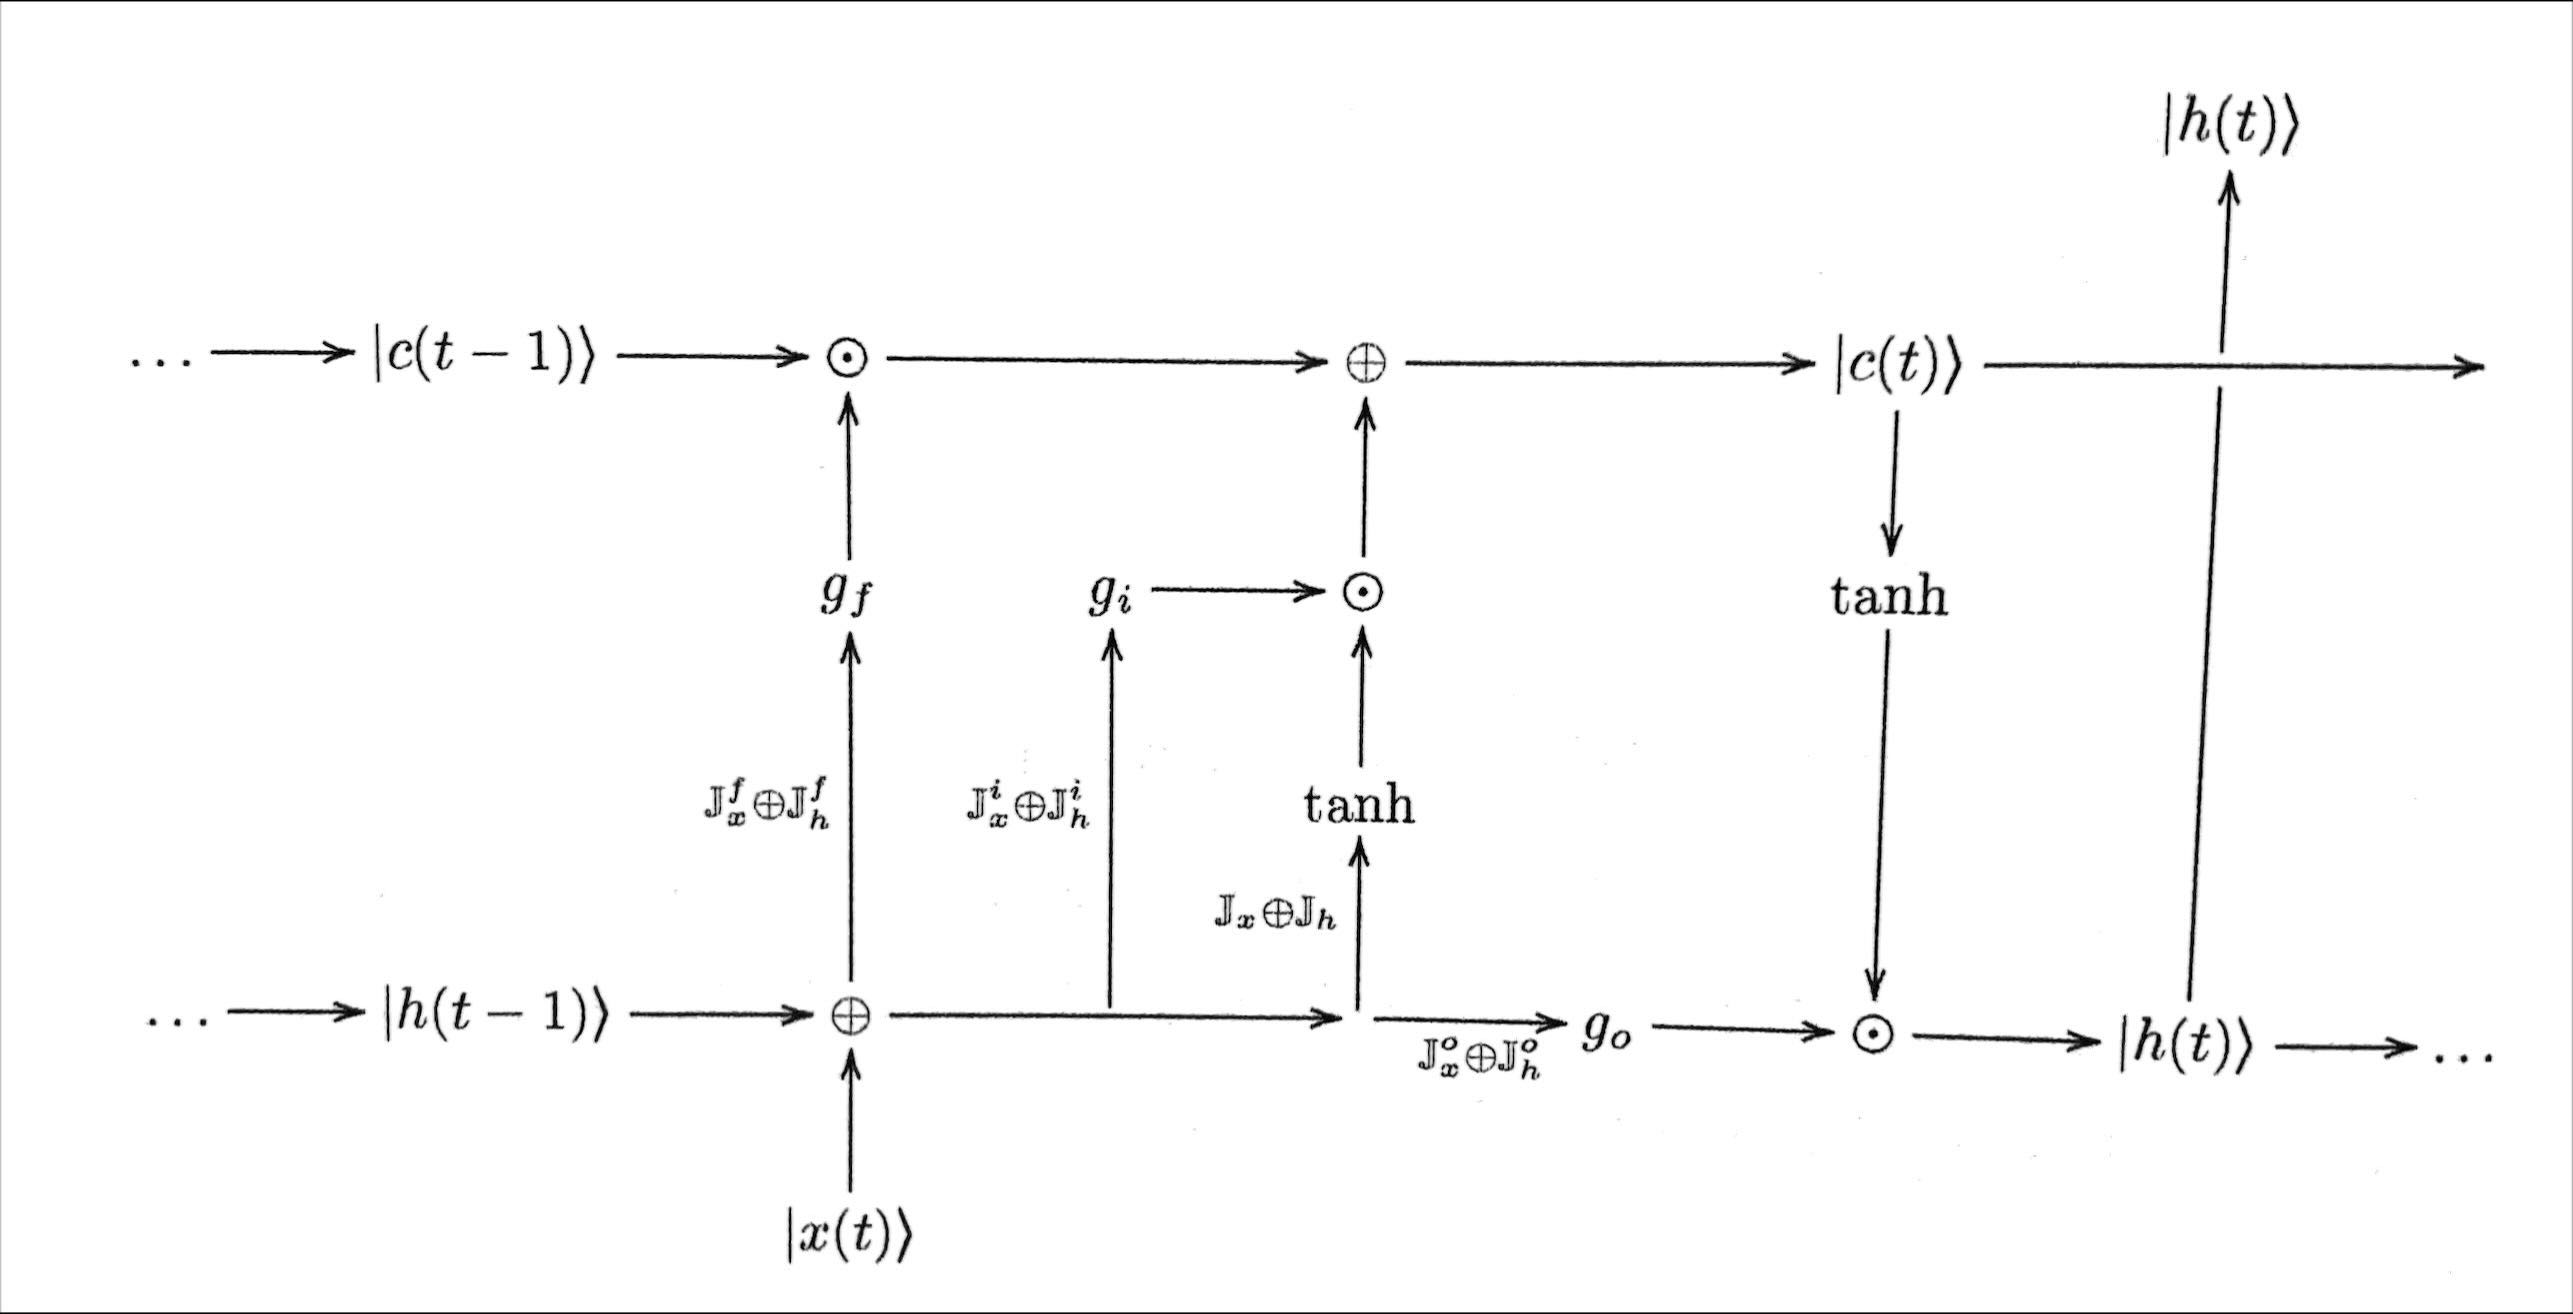
\includegraphics[height=5.7cm]{image/LSTM_diagram.jpeg}
      \end{center}
      \caption{LSTMの模式図.$\oplus$はベクトルの和,$\odot$はアダマール積を表す}
    \end{figure}
  \end{frame}

  \begin{frame}{LSTMの構造}
    LSTMの核心となるのはメモリベクトル$\ket{c(t)}$で,「一時的な記憶」を司る\\
    \vspace{0.3cm}
    $g_{\bullet}$はゲート(gate)であり,それぞれ
    \begin{align*}
      & g_f : \text{忘却ゲート}\\
      & g_i : \text{入力ゲート}\\
      & g_o : \text{出力ゲート}
    \end{align*}
    と呼ばれ,すべて成分ごとのシグモイド関数を取る
    \begin{equation*}
      g_f = g_i = g_o = \sigma
    \end{equation*}
  \end{frame}

  \begin{frame}{LSTMの構造}
    模式図から以下の関係式がわかる
    \begin{align*}
      \ket{h(t)} &= \sum_{m}\ket{m}\braket{m|g_o}\braket{m|\tanh{(c(t))}}\\ 
      \ket{c(t)} &= \sum_{m}\ket{m}\braket{m|c(t-1)}\braket{m|g_f}\\
      &+ \sum_m \ket{m}\tanh{\Big( \bra{m}\mathbb{J}_x \ket{x(t)} + \bra{m}\mathbb{J}_h \ket{h(t-1)} \Big)}\braket{m|g_i}\\
      \ket{g_f}  &= \sum_{m}\ket{m}g_f\Big( \bra{m}\mathbb{J}^{f}_{x}\ket{x(t)} + \bra{m}\mathbb{J}^{f}_{h}\ket{h(t-1)} \Big)\\
      \ket{g_i}  &= \sum_{m}\ket{m}g_i\Big( \bra{m}\mathbb{J}^{i}_{x}\ket{x(t)} + \bra{m}\mathbb{J}^{i}_{h}\ket{h(t-1)} \Big)\\
      \ket{g_o}  &= \sum_{m}\ket{m}g_o\Big( \bra{m}\mathbb{J}^{o}_{x}\ket{x(t)} + \bra{m}\mathbb{J}^{o}_{h}\ket{h(t-1)} \Big)
    \end{align*}
  \end{frame}

  \begin{frame}[t]{誤差逆伝播法}
    前節のRNNの時と同様の手順で誤差の逆伝播を見ていく\\
    \begin{equation*}
      \delta{h(t)} = \sum_{m}\Big[ \bra{m}\underbrace{\delta\ket{g_o}}_{\text{(A)}}\braket{m|\tanh{(c(t))}} + \braket{m|g_o}\bra{m}\underbrace{\delta \ket{\tanh{(c(t))}}}_{\text{(B)}} \Big]
    \end{equation*}
    まず,(A)について
    \begin{align*}
      (A) 
      &= \delta \sum_{m}\ket{m}g_o\Big( \bra{m}\mathbb{J}^{o}_{x}\ket{x(t)} + \bra{m}\mathbb{J}^{o}_{h}\ket{h(t-1)} \Big)\\
      &= \sum_{m}\ket{m}g'_{o}(\bullet)\Big[ \delta \Big( \bra{m}\mathbb{J}^{o}_{x}\ket{x(t)} + \bra{m}\mathbb{J}^{o}_{h}\ket{h(t-1)} \Big) \Big]\\
      &= \sum_{m}\ket{m}g'_{o}(\bullet)\Big[ \bra{m}\delta\mathbb{J}^{o}_{x}\ket{x(t)} + \bra{m}\delta\mathbb{J}^{o}_{h}\ket{h(t-1)} + \bra{m}\mathbb{J}^{o}_{h}\underbrace{\delta\ket{h(t-1)}}_{\bigstar}  \Big]
    \end{align*}
    $\bigstar$は時間をさかのぼって計算することができる.その際に$\mathbb{J}^{o}_{h}$が毎回1個ずつ出てくるので結局$\mathbb{J}^{o}_{h}$をたくさんかけることになり,勾配爆発/勾配消失が起こる
  \end{frame}

  \begin{frame}[t]{誤差逆伝播法}
    前節のRNNの時と同様の手順で誤差の逆伝播を見ていく\\
    \begin{equation*}
      \delta{h(t)} = \sum_{m}\Big[ \bra{m}\underbrace{\delta\ket{g_o}}_{\text{(A)}}\braket{m|\tanh{(c(t))}} + \braket{m|g_o}\bra{m}\underbrace{\delta \ket{\tanh{(c(t))}}}_{\text{(B)}} \Big]
    \end{equation*}
    次に,(B)について
    \begin{equation*}
      (B) = \delta\sum_{m}\ket{m}\tanh{(\braket{m|c(t)})} = \sum_{m}\ket{m}\tanh'{(\bullet)}\Big[ \bra{m}\underbrace{\delta\ket{c(t)}}_{\text{(C)}}  \Big]
    \end{equation*}
    勾配の大きさは(C)で決まる.計算すると
    \begin{align*}
      \text{(C)} 
      &= \sum_{m} \ket{m} \Big[ \bra{m}\delta\ket{c(t-1)}\braket{m|g_f} + \braket{m|c(t-1)}\bra{m}\underbrace{\delta\ket{g_f}}_{\text{(D)}} \Big]\\
      &+ \sum_{m} \ket{m}\Big[ \tanh'{(\bullet)}\Big( \bra{m}\delta\mathbb{J}_x\ket{x(t)} + \bra{m}\delta\mathbb{J}_h\ket{h(t-1)} + \bra{m}\mathbb{J}_h \delta\ket{h(t-1)} \Big)\braket{m|g_i}\\
      &+ \tanh{(\bullet)}\bra{m}\underbrace{\delta\ket{g_i}}_{\text{(F)}} \Big]
    \end{align*}
  \end{frame}

  \begin{frame}{(C)計算}
    \begin{align*}
      \text{(C)} 
      &= \delta\sum_{m}\ket{m}\braket{m|c(t-1)}\braket{m|g_f}\\
      &+ \delta\sum_m \ket{m}\tanh{\Big( \bra{m}\mathbb{J}_x \ket{x(t)} + \bra{m}\mathbb{J}_h \ket{h(t-1)} \Big)}\braket{m|g_i}\\ 
      &= \sum_{m} \ket{m} \Big[ \bra{m}\delta\ket{c(t-1)}\braket{m|g_f} + \braket{m|c(t-1)}\bra{m}\underbrace{\delta\ket{g_f}}_{\text{(D)}} \Big]\\
      &+ \sum_{m} \ket{m}\Big[ \tanh'{(\bullet)}\Big( \bra{m}\delta\mathbb{J}_x\ket{x(t)} + \bra{m}\delta\mathbb{J}_h\ket{h(t-1)} + \bra{m}\mathbb{J}_h \delta\ket{h(t-1)} \Big)\braket{m|g_i}\\
      &+ \tanh{(\bullet)}\bra{m}\underbrace{\delta\ket{g_i}}_{\text{(F)}} \Big]
    \end{align*}
    
  \end{frame}


\end{document}